% Options for packages loaded elsewhere
\PassOptionsToPackage{unicode}{hyperref}
\PassOptionsToPackage{hyphens}{url}
\PassOptionsToPackage{dvipsnames,svgnames,x11names}{xcolor}
%
\documentclass[
  letterpaper,
  DIV=11,
  numbers=noendperiod]{scrartcl}

\usepackage{amsmath,amssymb}
\usepackage{iftex}
\ifPDFTeX
  \usepackage[T1]{fontenc}
  \usepackage[utf8]{inputenc}
  \usepackage{textcomp} % provide euro and other symbols
\else % if luatex or xetex
  \usepackage{unicode-math}
  \defaultfontfeatures{Scale=MatchLowercase}
  \defaultfontfeatures[\rmfamily]{Ligatures=TeX,Scale=1}
\fi
\usepackage{lmodern}
\ifPDFTeX\else  
    % xetex/luatex font selection
\fi
% Use upquote if available, for straight quotes in verbatim environments
\IfFileExists{upquote.sty}{\usepackage{upquote}}{}
\IfFileExists{microtype.sty}{% use microtype if available
  \usepackage[]{microtype}
  \UseMicrotypeSet[protrusion]{basicmath} % disable protrusion for tt fonts
}{}
\makeatletter
\@ifundefined{KOMAClassName}{% if non-KOMA class
  \IfFileExists{parskip.sty}{%
    \usepackage{parskip}
  }{% else
    \setlength{\parindent}{0pt}
    \setlength{\parskip}{6pt plus 2pt minus 1pt}}
}{% if KOMA class
  \KOMAoptions{parskip=half}}
\makeatother
\usepackage{xcolor}
\setlength{\emergencystretch}{3em} % prevent overfull lines
\setcounter{secnumdepth}{-\maxdimen} % remove section numbering
% Make \paragraph and \subparagraph free-standing
\makeatletter
\ifx\paragraph\undefined\else
  \let\oldparagraph\paragraph
  \renewcommand{\paragraph}{
    \@ifstar
      \xxxParagraphStar
      \xxxParagraphNoStar
  }
  \newcommand{\xxxParagraphStar}[1]{\oldparagraph*{#1}\mbox{}}
  \newcommand{\xxxParagraphNoStar}[1]{\oldparagraph{#1}\mbox{}}
\fi
\ifx\subparagraph\undefined\else
  \let\oldsubparagraph\subparagraph
  \renewcommand{\subparagraph}{
    \@ifstar
      \xxxSubParagraphStar
      \xxxSubParagraphNoStar
  }
  \newcommand{\xxxSubParagraphStar}[1]{\oldsubparagraph*{#1}\mbox{}}
  \newcommand{\xxxSubParagraphNoStar}[1]{\oldsubparagraph{#1}\mbox{}}
\fi
\makeatother

\usepackage{color}
\usepackage{fancyvrb}
\newcommand{\VerbBar}{|}
\newcommand{\VERB}{\Verb[commandchars=\\\{\}]}
\DefineVerbatimEnvironment{Highlighting}{Verbatim}{commandchars=\\\{\}}
% Add ',fontsize=\small' for more characters per line
\usepackage{framed}
\definecolor{shadecolor}{RGB}{241,243,245}
\newenvironment{Shaded}{\begin{snugshade}}{\end{snugshade}}
\newcommand{\AlertTok}[1]{\textcolor[rgb]{0.68,0.00,0.00}{#1}}
\newcommand{\AnnotationTok}[1]{\textcolor[rgb]{0.37,0.37,0.37}{#1}}
\newcommand{\AttributeTok}[1]{\textcolor[rgb]{0.40,0.45,0.13}{#1}}
\newcommand{\BaseNTok}[1]{\textcolor[rgb]{0.68,0.00,0.00}{#1}}
\newcommand{\BuiltInTok}[1]{\textcolor[rgb]{0.00,0.23,0.31}{#1}}
\newcommand{\CharTok}[1]{\textcolor[rgb]{0.13,0.47,0.30}{#1}}
\newcommand{\CommentTok}[1]{\textcolor[rgb]{0.37,0.37,0.37}{#1}}
\newcommand{\CommentVarTok}[1]{\textcolor[rgb]{0.37,0.37,0.37}{\textit{#1}}}
\newcommand{\ConstantTok}[1]{\textcolor[rgb]{0.56,0.35,0.01}{#1}}
\newcommand{\ControlFlowTok}[1]{\textcolor[rgb]{0.00,0.23,0.31}{\textbf{#1}}}
\newcommand{\DataTypeTok}[1]{\textcolor[rgb]{0.68,0.00,0.00}{#1}}
\newcommand{\DecValTok}[1]{\textcolor[rgb]{0.68,0.00,0.00}{#1}}
\newcommand{\DocumentationTok}[1]{\textcolor[rgb]{0.37,0.37,0.37}{\textit{#1}}}
\newcommand{\ErrorTok}[1]{\textcolor[rgb]{0.68,0.00,0.00}{#1}}
\newcommand{\ExtensionTok}[1]{\textcolor[rgb]{0.00,0.23,0.31}{#1}}
\newcommand{\FloatTok}[1]{\textcolor[rgb]{0.68,0.00,0.00}{#1}}
\newcommand{\FunctionTok}[1]{\textcolor[rgb]{0.28,0.35,0.67}{#1}}
\newcommand{\ImportTok}[1]{\textcolor[rgb]{0.00,0.46,0.62}{#1}}
\newcommand{\InformationTok}[1]{\textcolor[rgb]{0.37,0.37,0.37}{#1}}
\newcommand{\KeywordTok}[1]{\textcolor[rgb]{0.00,0.23,0.31}{\textbf{#1}}}
\newcommand{\NormalTok}[1]{\textcolor[rgb]{0.00,0.23,0.31}{#1}}
\newcommand{\OperatorTok}[1]{\textcolor[rgb]{0.37,0.37,0.37}{#1}}
\newcommand{\OtherTok}[1]{\textcolor[rgb]{0.00,0.23,0.31}{#1}}
\newcommand{\PreprocessorTok}[1]{\textcolor[rgb]{0.68,0.00,0.00}{#1}}
\newcommand{\RegionMarkerTok}[1]{\textcolor[rgb]{0.00,0.23,0.31}{#1}}
\newcommand{\SpecialCharTok}[1]{\textcolor[rgb]{0.37,0.37,0.37}{#1}}
\newcommand{\SpecialStringTok}[1]{\textcolor[rgb]{0.13,0.47,0.30}{#1}}
\newcommand{\StringTok}[1]{\textcolor[rgb]{0.13,0.47,0.30}{#1}}
\newcommand{\VariableTok}[1]{\textcolor[rgb]{0.07,0.07,0.07}{#1}}
\newcommand{\VerbatimStringTok}[1]{\textcolor[rgb]{0.13,0.47,0.30}{#1}}
\newcommand{\WarningTok}[1]{\textcolor[rgb]{0.37,0.37,0.37}{\textit{#1}}}

\providecommand{\tightlist}{%
  \setlength{\itemsep}{0pt}\setlength{\parskip}{0pt}}\usepackage{longtable,booktabs,array}
\usepackage{calc} % for calculating minipage widths
% Correct order of tables after \paragraph or \subparagraph
\usepackage{etoolbox}
\makeatletter
\patchcmd\longtable{\par}{\if@noskipsec\mbox{}\fi\par}{}{}
\makeatother
% Allow footnotes in longtable head/foot
\IfFileExists{footnotehyper.sty}{\usepackage{footnotehyper}}{\usepackage{footnote}}
\makesavenoteenv{longtable}
\usepackage{graphicx}
\makeatletter
\def\maxwidth{\ifdim\Gin@nat@width>\linewidth\linewidth\else\Gin@nat@width\fi}
\def\maxheight{\ifdim\Gin@nat@height>\textheight\textheight\else\Gin@nat@height\fi}
\makeatother
% Scale images if necessary, so that they will not overflow the page
% margins by default, and it is still possible to overwrite the defaults
% using explicit options in \includegraphics[width, height, ...]{}
\setkeys{Gin}{width=\maxwidth,height=\maxheight,keepaspectratio}
% Set default figure placement to htbp
\makeatletter
\def\fps@figure{htbp}
\makeatother

\KOMAoption{captions}{tableheading}
\makeatletter
\@ifpackageloaded{caption}{}{\usepackage{caption}}
\AtBeginDocument{%
\ifdefined\contentsname
  \renewcommand*\contentsname{Table of contents}
\else
  \newcommand\contentsname{Table of contents}
\fi
\ifdefined\listfigurename
  \renewcommand*\listfigurename{List of Figures}
\else
  \newcommand\listfigurename{List of Figures}
\fi
\ifdefined\listtablename
  \renewcommand*\listtablename{List of Tables}
\else
  \newcommand\listtablename{List of Tables}
\fi
\ifdefined\figurename
  \renewcommand*\figurename{Figure}
\else
  \newcommand\figurename{Figure}
\fi
\ifdefined\tablename
  \renewcommand*\tablename{Table}
\else
  \newcommand\tablename{Table}
\fi
}
\@ifpackageloaded{float}{}{\usepackage{float}}
\floatstyle{ruled}
\@ifundefined{c@chapter}{\newfloat{codelisting}{h}{lop}}{\newfloat{codelisting}{h}{lop}[chapter]}
\floatname{codelisting}{Listing}
\newcommand*\listoflistings{\listof{codelisting}{List of Listings}}
\makeatother
\makeatletter
\makeatother
\makeatletter
\@ifpackageloaded{caption}{}{\usepackage{caption}}
\@ifpackageloaded{subcaption}{}{\usepackage{subcaption}}
\makeatother

\ifLuaTeX
  \usepackage{selnolig}  % disable illegal ligatures
\fi
\usepackage{bookmark}

\IfFileExists{xurl.sty}{\usepackage{xurl}}{} % add URL line breaks if available
\urlstyle{same} % disable monospaced font for URLs
\hypersetup{
  pdftitle={The Landscape of Renal Replacement Therapy in Nigeria \textbar{} 2022 - 2023},
  pdfauthor={Analysis by: Nelson Udeme-Abasi},
  colorlinks=true,
  linkcolor={blue},
  filecolor={Maroon},
  citecolor={Blue},
  urlcolor={Blue},
  pdfcreator={LaTeX via pandoc}}


\title{The Landscape of Renal Replacement Therapy in Nigeria \textbar{}
2022 - 2023}
\usepackage{etoolbox}
\makeatletter
\providecommand{\subtitle}[1]{% add subtitle to \maketitle
  \apptocmd{\@title}{\par {\large #1 \par}}{}{}
}
\makeatother
\subtitle{A project of the renal registry committee of the Nigerian
Association of Nephrologists}
\author{Analysis by: Nelson Udeme-Abasi}
\date{}

\begin{document}
\maketitle


\section{Analysis}\label{analysis}

\subsection{Summary Statistics}\label{summary-statistics}

Loading necessary packages and loading the data

\begin{Shaded}
\begin{Highlighting}[]
\CommentTok{\# Loading the necessary packages}
\FunctionTok{library}\NormalTok{(tidyverse)}
\FunctionTok{library}\NormalTok{(gtsummary)}
\FunctionTok{library}\NormalTok{(gt)}
\FunctionTok{library}\NormalTok{(ggplot2)}
\FunctionTok{library}\NormalTok{(survival)}
\FunctionTok{library}\NormalTok{(survminer)}
\FunctionTok{library}\NormalTok{(sf)}
\FunctionTok{library}\NormalTok{(ggspatial)}
\FunctionTok{library}\NormalTok{(prettymapr)}
\FunctionTok{library}\NormalTok{(labelled)}

\CommentTok{\# Loading the data}
\NormalTok{rr\_data }\OtherTok{\textless{}{-}} \FunctionTok{read\_csv}\NormalTok{(}\StringTok{\textquotesingle{}rr\_data.csv\textquotesingle{}}\NormalTok{, }\AttributeTok{trim\_ws =}\NormalTok{ T)}
\end{Highlighting}
\end{Shaded}

\begin{itemize}
\item
  Selecting the necessary columns for my analysis and enforcing data
  types
\item
  Adding necessary columns
\item
  Forcing data types to ease analysis
\end{itemize}

\begin{Shaded}
\begin{Highlighting}[]
\NormalTok{rr\_data\_new }\OtherTok{\textless{}{-}}\NormalTok{ rr\_data }\SpecialCharTok{\%\textgreater{}\%} 
  \FunctionTok{select}\NormalTok{(}\FunctionTok{c}\NormalTok{(Sex, Age, Zone, State, }\StringTok{\textasciigrave{}}\AttributeTok{Centre Category}\StringTok{\textasciigrave{}}\NormalTok{, }\StringTok{\textasciigrave{}}\AttributeTok{First Modality}\StringTok{\textasciigrave{}}\NormalTok{, }\StringTok{\textasciigrave{}}\AttributeTok{Vascular Access}\StringTok{\textasciigrave{}}\NormalTok{, DM, HBV, HIV, HCV, Outcome, }\StringTok{\textasciigrave{}}\AttributeTok{Date of Diagnosis}\StringTok{\textasciigrave{}}\NormalTok{, }\StringTok{\textasciigrave{}}\AttributeTok{Date of Death or Transplant}\StringTok{\textasciigrave{}}\NormalTok{))}

\CommentTok{\# Creating labels for my table columns}
\NormalTok{col\_labels }\OtherTok{\textless{}{-}} \FunctionTok{c}\NormalTok{(}\StringTok{\textquotesingle{}Sex\textquotesingle{}}\NormalTok{, }\StringTok{\textquotesingle{}Age(years)\textquotesingle{}}\NormalTok{,}\StringTok{\textquotesingle{}Geopolitical Zone\textquotesingle{}}\NormalTok{, }\StringTok{\textquotesingle{}State\textquotesingle{}}\NormalTok{, }\StringTok{\textquotesingle{}Facility Type\textquotesingle{}}\NormalTok{, }\StringTok{\textquotesingle{}First Modality\textquotesingle{}}\NormalTok{,}\StringTok{\textquotesingle{}Vascular Access\textquotesingle{}}\NormalTok{, }\StringTok{\textquotesingle{}DM Status\textquotesingle{}}\NormalTok{, }\StringTok{\textquotesingle{}HBV Status\textquotesingle{}}\NormalTok{, }\StringTok{\textquotesingle{}HIV Status\textquotesingle{}}\NormalTok{, }\StringTok{\textquotesingle{}HCV Status\textquotesingle{}}\NormalTok{, }\StringTok{\textquotesingle{}Outcomes\textquotesingle{}}\NormalTok{, }\StringTok{\textquotesingle{}Date Diagnosed\textquotesingle{}}\NormalTok{, }\StringTok{\textquotesingle{}Date of Death or Transplant\textquotesingle{}}\NormalTok{)}

\NormalTok{rr\_data\_new }\OtherTok{\textless{}{-}} \FunctionTok{set\_variable\_labels}\NormalTok{(}\AttributeTok{.data =}\NormalTok{ rr\_data\_new, }\AttributeTok{.labels =}\NormalTok{ col\_labels)}

\NormalTok{rr\_data\_new }\OtherTok{\textless{}{-}}\NormalTok{ rr\_data\_new }\SpecialCharTok{\%\textgreater{}\%}
  \FunctionTok{mutate}\NormalTok{(}\StringTok{\textquotesingle{}Age Group\textquotesingle{}} \OtherTok{=} \FunctionTok{case\_when}\NormalTok{(Age }\SpecialCharTok{\textless{}} \DecValTok{20} \SpecialCharTok{\textasciitilde{}} \StringTok{\textquotesingle{}Less than 20\textquotesingle{}}\NormalTok{,}
\NormalTok{                                 Age }\SpecialCharTok{\textgreater{}=} \DecValTok{20} \SpecialCharTok{\&}\NormalTok{ Age }\SpecialCharTok{\textless{}=} \DecValTok{45} \SpecialCharTok{\textasciitilde{}} \StringTok{\textquotesingle{}20 to 45\textquotesingle{}}\NormalTok{,}
\NormalTok{                                 Age }\SpecialCharTok{\textgreater{}} \DecValTok{45} \SpecialCharTok{\&}\NormalTok{ Age }\SpecialCharTok{\textless{}=}\DecValTok{65} \SpecialCharTok{\textasciitilde{}} \StringTok{\textquotesingle{}46 to 65\textquotesingle{}}\NormalTok{,}
\NormalTok{                                 Age }\SpecialCharTok{\textgreater{}} \DecValTok{65} \SpecialCharTok{\textasciitilde{}} \StringTok{\textquotesingle{}Greater than 65\textquotesingle{}}\NormalTok{)}
\NormalTok{         ) }\SpecialCharTok{\%\textgreater{}\%} 
  \FunctionTok{mutate\_at}\NormalTok{(}\FunctionTok{c}\NormalTok{(}\StringTok{\textquotesingle{}Date of Diagnosis\textquotesingle{}}\NormalTok{,}\StringTok{\textquotesingle{}Date of Death or Transplant\textquotesingle{}}\NormalTok{), mdy) }\SpecialCharTok{\%\textgreater{}\%} 
  \FunctionTok{mutate\_at}\NormalTok{(}\FunctionTok{c}\NormalTok{(}\StringTok{\textquotesingle{}Sex\textquotesingle{}}\NormalTok{, }\StringTok{\textquotesingle{}Age Group\textquotesingle{}}\NormalTok{, }\StringTok{\textquotesingle{}Zone\textquotesingle{}}\NormalTok{, }\StringTok{\textquotesingle{}Centre Category\textquotesingle{}}\NormalTok{, }\StringTok{\textquotesingle{}First Modality\textquotesingle{}}\NormalTok{, }\StringTok{\textquotesingle{}Vascular Access\textquotesingle{}}\NormalTok{, }\StringTok{\textquotesingle{}DM\textquotesingle{}}\NormalTok{, }\StringTok{\textquotesingle{}HBV\textquotesingle{}}\NormalTok{, }\StringTok{\textquotesingle{}HCV\textquotesingle{}}\NormalTok{, }\StringTok{\textquotesingle{}HIV\textquotesingle{}}\NormalTok{, }\StringTok{\textquotesingle{}Outcome\textquotesingle{}}\NormalTok{), as.factor)}

\FunctionTok{head}\NormalTok{(rr\_data\_new)}
\end{Highlighting}
\end{Shaded}

\begin{verbatim}
# A tibble: 6 x 15
  Sex     Age Zone  State `Centre Category` `First Modality` `Vascular Access`  
  <fct> <dbl> <fct> <chr> <fct>             <fct>            <fct>              
1 M        73 SW    Ekiti Public            HD               Tunneled CVC       
2 M        60 SW    Ekiti Public            HD               Tunneled CVC       
3 F        35 SW    Ekiti Public            HD               Temporary Femoral ~
4 M        48 SW    Ekiti Public            HD               Tunneled CVC       
5 M        46 SW    Ekiti Public            HD               Temporary Femoral ~
6 M        30 SW    Ekiti Public            HD               Tunneled CVC       
# i 8 more variables: DM <fct>, HBV <fct>, HIV <fct>, HCV <fct>, Outcome <fct>,
#   `Date of Diagnosis` <date>, `Date of Death or Transplant` <date>,
#   `Age Group` <fct>
\end{verbatim}

Re-level factor variables to make sense of the data

\begin{Shaded}
\begin{Highlighting}[]
\NormalTok{rr\_data\_new }\OtherTok{\textless{}{-}}\NormalTok{ rr\_data\_new }\SpecialCharTok{\%\textgreater{}\%} 
  \FunctionTok{mutate}\NormalTok{(}\StringTok{\textasciigrave{}}\AttributeTok{Age Group}\StringTok{\textasciigrave{}} \OtherTok{=} \FunctionTok{fct\_relevel}\NormalTok{(}\StringTok{\textasciigrave{}}\AttributeTok{Age Group}\StringTok{\textasciigrave{}}\NormalTok{, }\StringTok{\textquotesingle{}Less than 20\textquotesingle{}}\NormalTok{,}\StringTok{\textquotesingle{}20 to 45\textquotesingle{}}\NormalTok{,}\StringTok{\textquotesingle{}46 to 65\textquotesingle{}}\NormalTok{, }\StringTok{\textquotesingle{}Greater than 65\textquotesingle{}}\NormalTok{), }
         \AttributeTok{DM =} \FunctionTok{fct\_relevel}\NormalTok{(DM, }\StringTok{\textquotesingle{}Yes\textquotesingle{}}\NormalTok{, }\StringTok{\textquotesingle{}No\textquotesingle{}}\NormalTok{),}
         \AttributeTok{HIV =} \FunctionTok{fct\_relevel}\NormalTok{(HIV, }\StringTok{\textquotesingle{}Pos\textquotesingle{}}\NormalTok{, }\StringTok{\textquotesingle{}Neg\textquotesingle{}}\NormalTok{),}
         \AttributeTok{HBV =} \FunctionTok{fct\_relevel}\NormalTok{(HBV, }\StringTok{\textquotesingle{}Pos\textquotesingle{}}\NormalTok{, }\StringTok{\textquotesingle{}Neg\textquotesingle{}}\NormalTok{),}
         \AttributeTok{HCV =} \FunctionTok{fct\_relevel}\NormalTok{(HCV, }\StringTok{\textquotesingle{}Pos\textquotesingle{}}\NormalTok{, }\StringTok{\textquotesingle{}Neg\textquotesingle{}}\NormalTok{),}
         \AttributeTok{Outcome =} \FunctionTok{fct\_relevel}\NormalTok{(Outcome, }\StringTok{\textquotesingle{}Dead\textquotesingle{}}\NormalTok{, }\StringTok{\textquotesingle{}Alive\textquotesingle{}}\NormalTok{, }\StringTok{\textquotesingle{}Transplant\textquotesingle{}}\NormalTok{)}
\NormalTok{         )}
\end{Highlighting}
\end{Shaded}

Below is the summary table of the patient's demographics

\begin{Shaded}
\begin{Highlighting}[]
\CommentTok{\#tbl\_summary(rr\_data\_new,}
\CommentTok{\# include = c(Sex, Age, \textasciigrave{}Age Group\textasciigrave{}, Zone, \textasciigrave{}Centre Category\textasciigrave{}),}
\CommentTok{\#  statistic = list(}
\CommentTok{\#    all\_continuous() \textasciitilde{} \textquotesingle{}\{median\} (\{p25\}, \{p75\})\textquotesingle{},}
\CommentTok{\#    all\_categorical() \textasciitilde{} \textquotesingle{}\{n\} (\{p\}\%)\textquotesingle{}}
\CommentTok{\#  ),}
\CommentTok{\#  digits = list(}
\CommentTok{\#    all\_categorical() \textasciitilde{} c(0, 1),}
\CommentTok{\#    all\_continuous() \textasciitilde{} c(1,1)}
\CommentTok{\#  )}
\CommentTok{\#  ) \%\textgreater{}\% }
\CommentTok{\#  modify\_header(label \textasciitilde{} \textquotesingle{}**Variables**\textquotesingle{}) \%\textgreater{}\% }
\CommentTok{\#  modify\_caption(\textquotesingle{}**Table 1 Sociodemographic Characteristics of Patients**\textquotesingle{}) \%\textgreater{}\% }
\CommentTok{\#  bold\_labels() \%\textgreater{}\% }
\CommentTok{\#  as\_gt() \%\textgreater{}\% }
\CommentTok{\#  cols\_width(everything() \textasciitilde{} px(250))}
\CommentTok{\#  )}
\end{Highlighting}
\end{Shaded}

\subsection{Geographical Distribution of Patients (using the UN human
data Nigerian shape
file)}\label{geographical-distribution-of-patients-using-the-un-human-data-nigerian-shape-file}

\begin{Shaded}
\begin{Highlighting}[]
\CommentTok{\# Bring in the UN human data Nigerian shape file and merge/join with the relevant summary in the data}

\NormalTok{nigeria }\OtherTok{\textless{}{-}} \FunctionTok{read\_sf}\NormalTok{(}\StringTok{\textquotesingle{}nga\_admbnda\_adm1\_osgof\_20190417.shp\textquotesingle{}}\NormalTok{)}

\CommentTok{\# Creating a summary of all states with patient\textquotesingle{}s number}

\NormalTok{pts\_geog\_distr }\OtherTok{\textless{}{-}}\NormalTok{ rr\_data\_new }\SpecialCharTok{\%\textgreater{}\%} 
  \FunctionTok{group\_by}\NormalTok{(State) }\SpecialCharTok{\%\textgreater{}\%} 
  \FunctionTok{summarise}\NormalTok{(}\AttributeTok{pts\_per\_state =} \FunctionTok{n}\NormalTok{()) }\SpecialCharTok{\%\textgreater{}\%} 
  \FunctionTok{ungroup}\NormalTok{()}

\FunctionTok{head}\NormalTok{(pts\_geog\_distr)}
\end{Highlighting}
\end{Shaded}

\begin{verbatim}
# A tibble: 6 x 2
  State       pts_per_state
  <chr>               <int>
1 Abia                  116
2 Akwa Ibom             201
3 Borno                  86
4 Cross River           135
5 Delta                  84
6 Ebonyi                 79
\end{verbatim}

\begin{Shaded}
\begin{Highlighting}[]
\CommentTok{\# Confirm columns in State are similar to ADM1\_EN}

\FunctionTok{anti\_join}\NormalTok{(pts\_geog\_distr, nigeria, }\AttributeTok{by =} \FunctionTok{c}\NormalTok{(}\StringTok{\textquotesingle{}State\textquotesingle{}} \OtherTok{=} \StringTok{\textquotesingle{}ADM1\_EN\textquotesingle{}}\NormalTok{))}
\end{Highlighting}
\end{Shaded}

\begin{verbatim}
# A tibble: 1 x 2
  State pts_per_state
  <chr>         <int>
1 FCT             937
\end{verbatim}

\begin{Shaded}
\begin{Highlighting}[]
\CommentTok{\# Only FCT is not named in the same way}

\CommentTok{\# So we will rename FCT in the pts\_geog\_distr df}
\NormalTok{pts\_geog\_distr }\OtherTok{\textless{}{-}}\NormalTok{ pts\_geog\_distr }\SpecialCharTok{\%\textgreater{}\%} 
  \FunctionTok{mutate}\NormalTok{(}\AttributeTok{State =} \FunctionTok{case\_when}\NormalTok{(State }\SpecialCharTok{==} \StringTok{\textquotesingle{}FCT\textquotesingle{}} \SpecialCharTok{\textasciitilde{}} \StringTok{\textquotesingle{}Federal Capital Territory\textquotesingle{}}\NormalTok{,}
                           \ConstantTok{TRUE} \SpecialCharTok{\textasciitilde{}}\NormalTok{ State)}
\NormalTok{         )}
\NormalTok{pts\_geog\_distr}
\end{Highlighting}
\end{Shaded}

\begin{verbatim}
# A tibble: 25 x 2
   State                     pts_per_state
   <chr>                             <int>
 1 Abia                                116
 2 Akwa Ibom                           201
 3 Borno                                86
 4 Cross River                         135
 5 Delta                                84
 6 Ebonyi                               79
 7 Ekiti                               103
 8 Enugu                               275
 9 Federal Capital Territory           937
10 Imo                                  14
# i 15 more rows
\end{verbatim}

\begin{Shaded}
\begin{Highlighting}[]
\CommentTok{\# Now safely combine both with a left join}

\NormalTok{map\_data }\OtherTok{\textless{}{-}} \FunctionTok{left\_join}\NormalTok{(nigeria, pts\_geog\_distr, }\AttributeTok{by =} \FunctionTok{c}\NormalTok{(}\StringTok{\textquotesingle{}ADM1\_EN\textquotesingle{}} \OtherTok{=} \StringTok{\textquotesingle{}State\textquotesingle{}}\NormalTok{))}
\end{Highlighting}
\end{Shaded}

Below is the map of \texttt{Nigeria} showing the state-level
geographical distribution of patients who underwent RRT in 2022 - 2023

\begin{Shaded}
\begin{Highlighting}[]
\CommentTok{\#compute cenntroids for states label}
\NormalTok{state\_centroids }\OtherTok{\textless{}{-}}\NormalTok{ map\_data }\SpecialCharTok{\%\textgreater{}\%}
  \FunctionTok{mutate}\NormalTok{(}\AttributeTok{centroid =} \FunctionTok{st\_centroid}\NormalTok{(geometry)) }\SpecialCharTok{\%\textgreater{}\%}
  \FunctionTok{mutate}\NormalTok{(}\AttributeTok{long =} \FunctionTok{st\_coordinates}\NormalTok{(centroid)[,}\DecValTok{1}\NormalTok{],}
         \AttributeTok{lat  =} \FunctionTok{st\_coordinates}\NormalTok{(centroid)[,}\DecValTok{2}\NormalTok{])}

\CommentTok{\# Now plot the map}
\NormalTok{map\_data }\SpecialCharTok{\%\textgreater{}\%} 
  \FunctionTok{ggplot}\NormalTok{(}\FunctionTok{aes}\NormalTok{(}\AttributeTok{fill =}\NormalTok{ pts\_per\_state)) }\SpecialCharTok{+}
  \FunctionTok{geom\_sf}\NormalTok{()}\SpecialCharTok{+}
  \FunctionTok{geom\_point}\NormalTok{(}\AttributeTok{data =}\NormalTok{ state\_centroids, }\FunctionTok{aes}\NormalTok{(}\AttributeTok{x =}\NormalTok{ long, }\AttributeTok{y =}\NormalTok{ lat))}\SpecialCharTok{+}
  \FunctionTok{geom\_text}\NormalTok{(}\AttributeTok{data =}\NormalTok{ state\_centroids, }\FunctionTok{aes}\NormalTok{(}\AttributeTok{x =}\NormalTok{ long, }\AttributeTok{y =}\NormalTok{ lat, }\AttributeTok{label =}\NormalTok{ ADM1\_EN),}
            \AttributeTok{size =} \DecValTok{3}\NormalTok{, }\AttributeTok{color =} \StringTok{"black"}\NormalTok{, }\AttributeTok{nudge\_y =} \SpecialCharTok{{-}}\NormalTok{.}\DecValTok{2}\NormalTok{) }\SpecialCharTok{+}
  \FunctionTok{scale\_fill\_gradient}\NormalTok{(}
    \AttributeTok{low =} \StringTok{"\#d8f3dc"}\NormalTok{, }\AttributeTok{high =} \StringTok{"\#00A676"}\NormalTok{, }\AttributeTok{na.value =} \StringTok{"grey90"}\NormalTok{)}\SpecialCharTok{+}
  \FunctionTok{labs}\NormalTok{(}
    \AttributeTok{title =} \StringTok{"Geographical distribution of patients by State"}\NormalTok{,}
    \AttributeTok{caption =} \StringTok{"Nigerian shapefile: gotten from humandata.org"}
\NormalTok{  ) }\SpecialCharTok{+}
  \FunctionTok{theme\_bw}\NormalTok{()}
\end{Highlighting}
\end{Shaded}

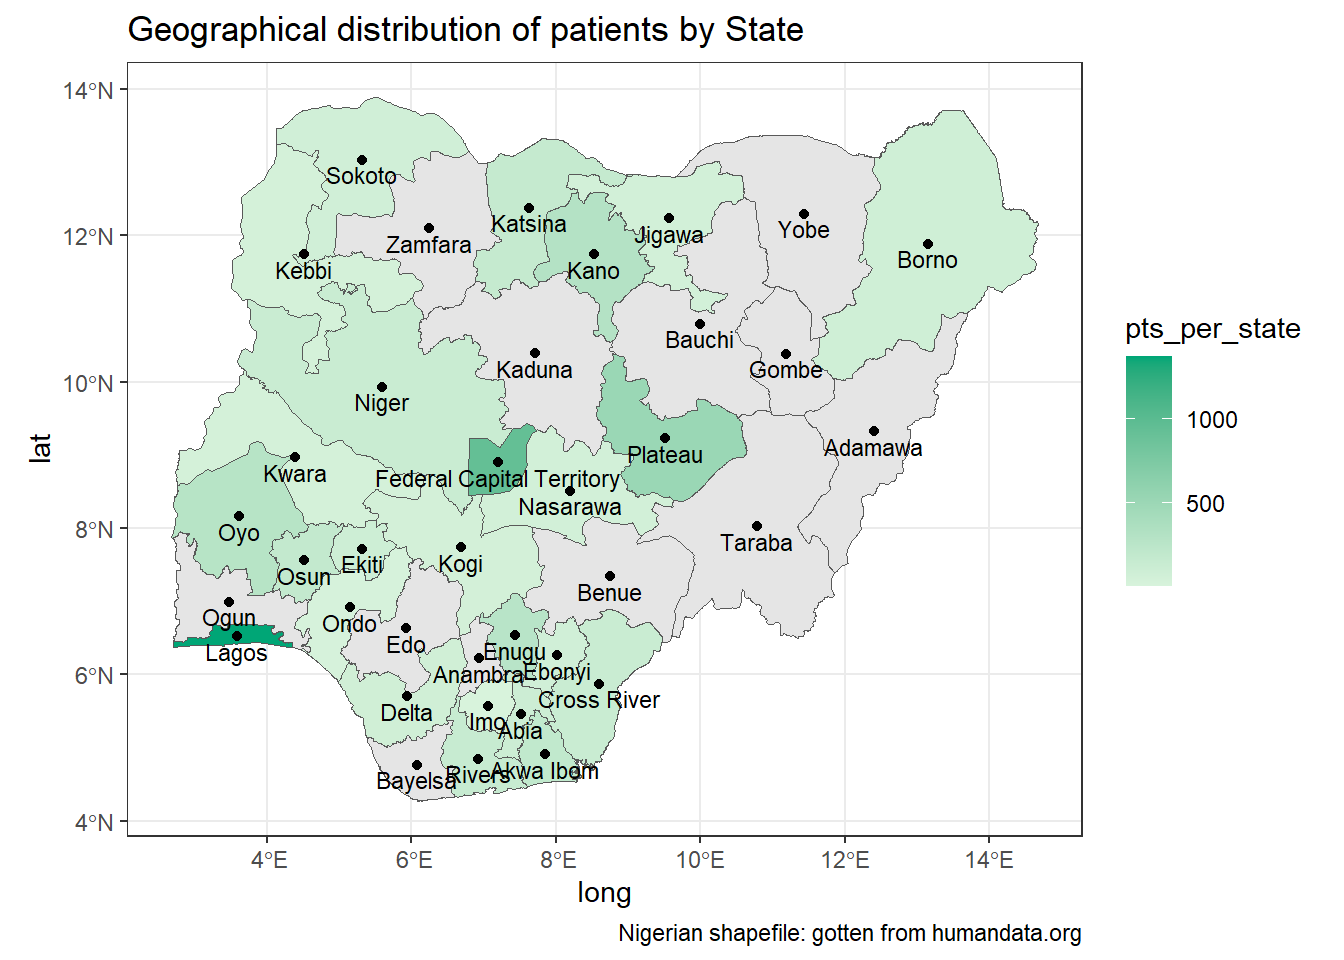
\includegraphics{nationalRR_files/figure-pdf/unnamed-chunk-8-1.pdf}

\subsection{Patient's Distribution by Facility Type and
Zone}\label{patients-distribution-by-facility-type-and-zone}

Below is the patient distribution by facility category and zone

\begin{Shaded}
\begin{Highlighting}[]
\NormalTok{rr\_data\_new }\SpecialCharTok{\%\textgreater{}\%} 
  \FunctionTok{group\_by}\NormalTok{(Zone, }\StringTok{\textasciigrave{}}\AttributeTok{Centre Category}\StringTok{\textasciigrave{}}\NormalTok{) }\SpecialCharTok{\%\textgreater{}\%} 
  \FunctionTok{summarise}\NormalTok{(}\StringTok{\textquotesingle{}No of Patients\textquotesingle{}} \OtherTok{=} \FunctionTok{n}\NormalTok{()) }\SpecialCharTok{\%\textgreater{}\%} 
    \FunctionTok{ggplot}\NormalTok{(}\FunctionTok{aes}\NormalTok{(}\AttributeTok{x =}\NormalTok{ Zone, }\AttributeTok{y =} \StringTok{\textasciigrave{}}\AttributeTok{No of Patients}\StringTok{\textasciigrave{}}\NormalTok{, }\AttributeTok{fill =} \StringTok{\textasciigrave{}}\AttributeTok{Centre Category}\StringTok{\textasciigrave{}}\NormalTok{, }\AttributeTok{width =}\NormalTok{ .}\DecValTok{7}\NormalTok{))}\SpecialCharTok{+}
      \FunctionTok{geom\_bar}\NormalTok{(}\AttributeTok{stat =} \StringTok{\textquotesingle{}identity\textquotesingle{}}\NormalTok{, }\AttributeTok{position =} \FunctionTok{position\_dodge}\NormalTok{(}\AttributeTok{width =} \FloatTok{0.75}\NormalTok{, }\AttributeTok{preserve =} \StringTok{"single"}\NormalTok{))}\SpecialCharTok{+}
      \FunctionTok{scale\_fill\_manual}\NormalTok{(}\AttributeTok{values =} \FunctionTok{c}\NormalTok{(}\StringTok{"Private"} \OtherTok{=} \StringTok{"\#E97132"}\NormalTok{, }\StringTok{"Public"} \OtherTok{=} \StringTok{"\#00A676"}\NormalTok{)) }\SpecialCharTok{+}
      \FunctionTok{labs}\NormalTok{(}\AttributeTok{title =} \StringTok{\textquotesingle{}\textquotesingle{}}\NormalTok{)}\SpecialCharTok{+}
      \FunctionTok{theme\_bw}\NormalTok{()}
\end{Highlighting}
\end{Shaded}

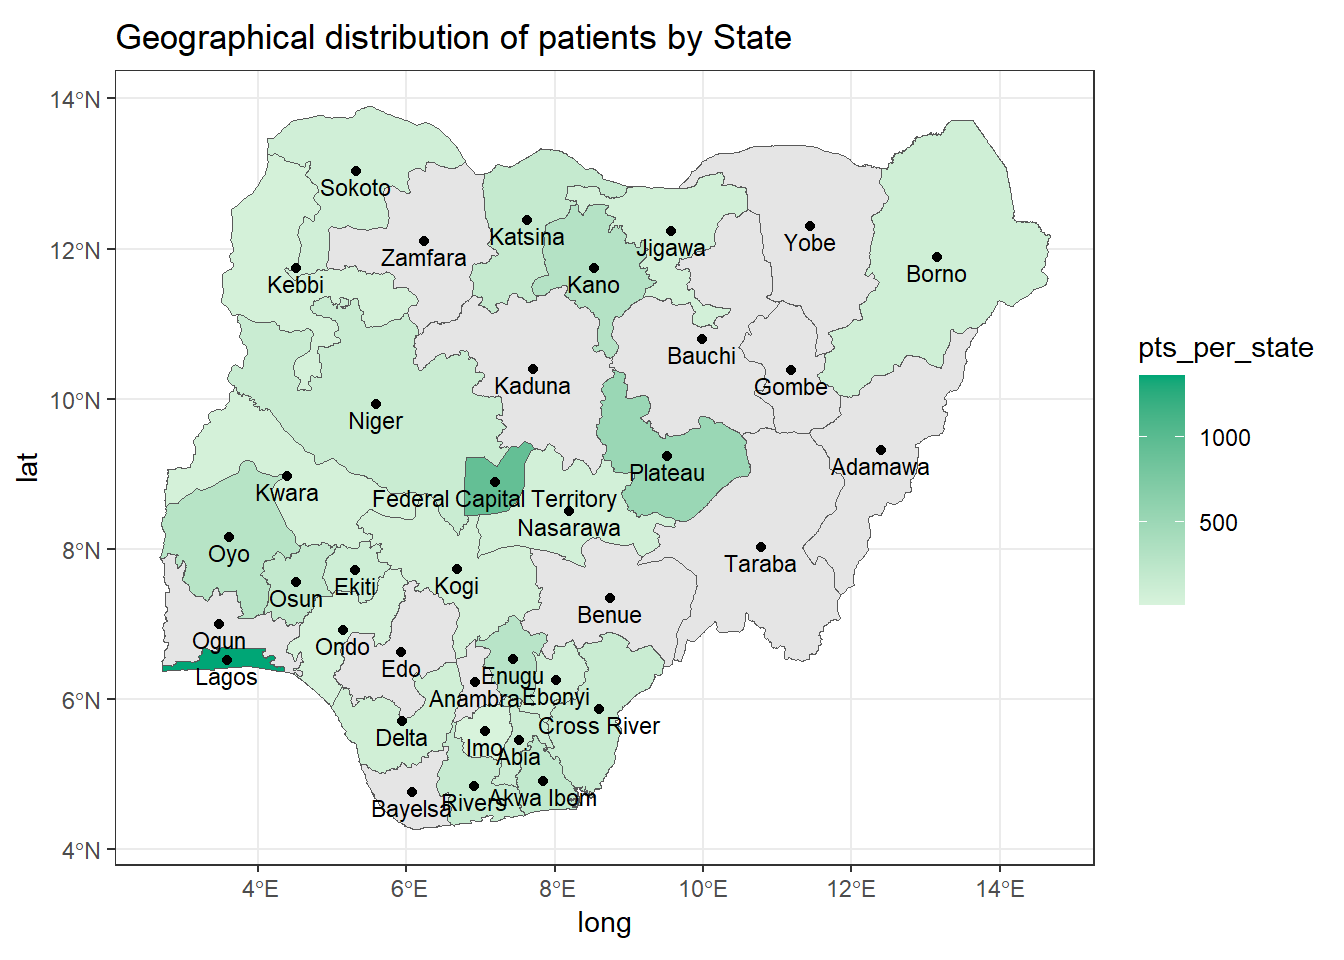
\includegraphics{nationalRR_files/figure-pdf/unnamed-chunk-9-1.pdf}

\subsection{Age Distribution by Zone and
Category}\label{age-distribution-by-zone-and-category}

\begin{Shaded}
\begin{Highlighting}[]
\FunctionTok{ggplot}\NormalTok{(}\AttributeTok{data =}\NormalTok{ rr\_data\_new, }\FunctionTok{aes}\NormalTok{(}\AttributeTok{x =}\NormalTok{ Zone, }\AttributeTok{y =}\NormalTok{ Age, }\AttributeTok{fill =} \StringTok{\textasciigrave{}}\AttributeTok{Centre Category}\StringTok{\textasciigrave{}}\NormalTok{))}\SpecialCharTok{+}
  \FunctionTok{stat\_boxplot}\NormalTok{(}\AttributeTok{geom =} \StringTok{"errorbar"}\NormalTok{,}
               \AttributeTok{position =} \FunctionTok{position\_dodge}\NormalTok{(}\AttributeTok{width =} \FloatTok{0.75}\NormalTok{, }\AttributeTok{preserve =} \StringTok{"single"}\NormalTok{),}
               \AttributeTok{width =} \FloatTok{0.2}
\NormalTok{               )}\SpecialCharTok{+}
  \FunctionTok{annotate}\NormalTok{(}\StringTok{"rect"}\NormalTok{, }\AttributeTok{xmin =} \SpecialCharTok{{-}}\ConstantTok{Inf}\NormalTok{, }\AttributeTok{xmax =} \ConstantTok{Inf}\NormalTok{, }\AttributeTok{ymin =} \DecValTok{40}\NormalTok{, }\AttributeTok{ymax =} \DecValTok{60}\NormalTok{, }
           \AttributeTok{fill =} \StringTok{"\#FF0000"}\NormalTok{, }\AttributeTok{alpha =} \FloatTok{0.3}\NormalTok{) }\SpecialCharTok{+}
  \FunctionTok{geom\_boxplot}\NormalTok{(}\AttributeTok{position =} \FunctionTok{position\_dodge}\NormalTok{(}\AttributeTok{width =} \FloatTok{0.75}\NormalTok{, }\AttributeTok{preserve =} \StringTok{"single"}\NormalTok{), }\AttributeTok{width =}\NormalTok{ .}\DecValTok{6}\NormalTok{)}\SpecialCharTok{+}
  \FunctionTok{scale\_fill\_manual}\NormalTok{(}\AttributeTok{values =} \FunctionTok{c}\NormalTok{(}\StringTok{"Private"} \OtherTok{=} \StringTok{"\#E97132"}\NormalTok{, }\StringTok{"Public"} \OtherTok{=} \StringTok{"\#00A676"}\NormalTok{))}\SpecialCharTok{+}
  \FunctionTok{geom\_hline}\NormalTok{(}\AttributeTok{yintercept =} \DecValTok{60}\NormalTok{, }\AttributeTok{linetype =} \StringTok{\textquotesingle{}dashed\textquotesingle{}}\NormalTok{)}\SpecialCharTok{+}
  \FunctionTok{geom\_hline}\NormalTok{(}\AttributeTok{yintercept =} \DecValTok{40}\NormalTok{, }\AttributeTok{linetype =} \StringTok{\textquotesingle{}dashed\textquotesingle{}}\NormalTok{)}\SpecialCharTok{+}
    \FunctionTok{theme\_bw}\NormalTok{()}
\end{Highlighting}
\end{Shaded}

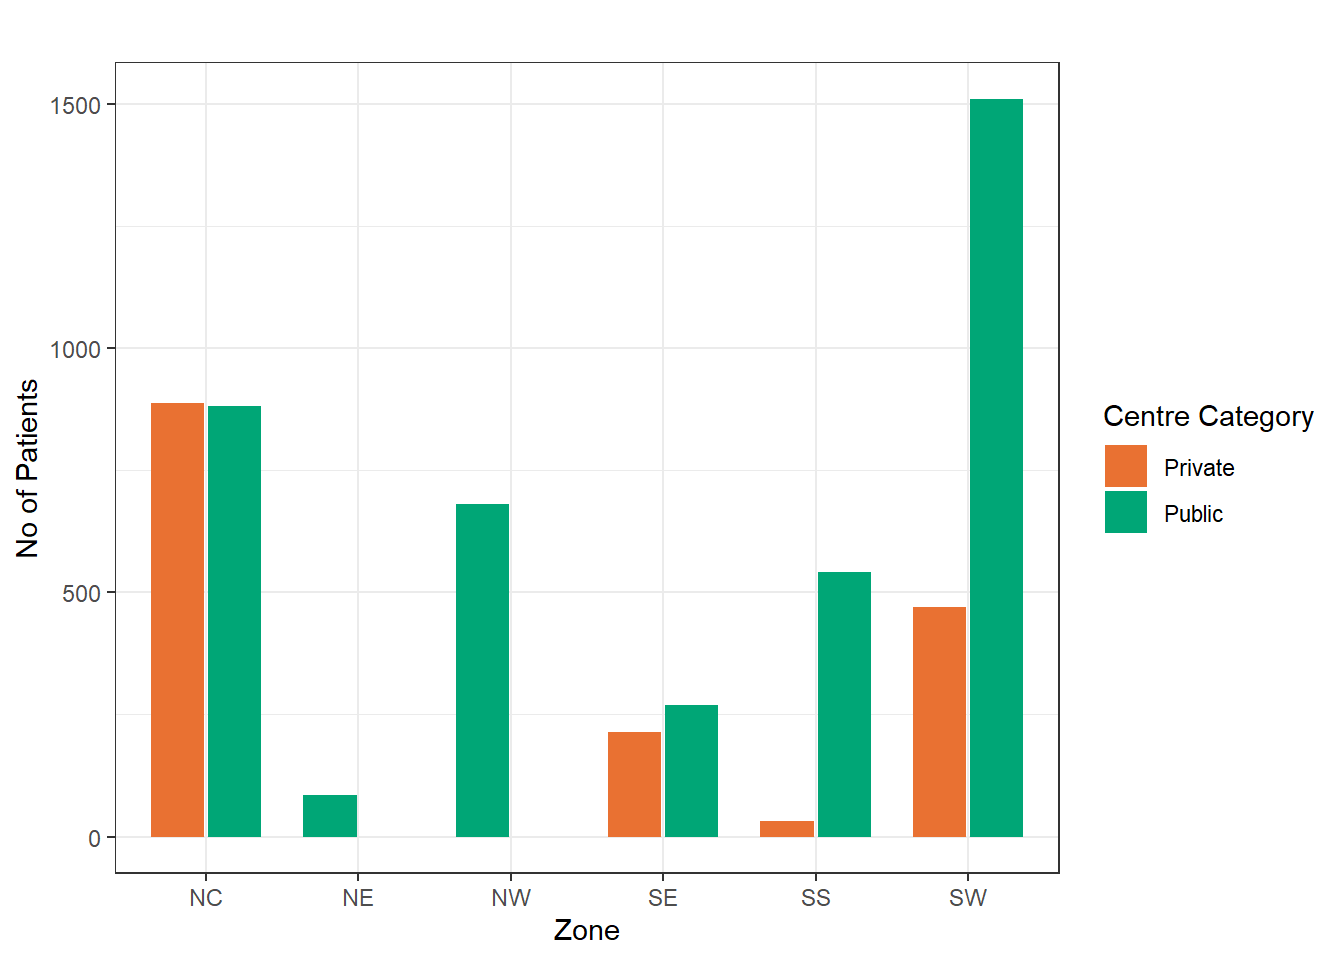
\includegraphics{nationalRR_files/figure-pdf/unnamed-chunk-10-1.pdf}

\subsection{Patients Distribution by Sex and
Zone}\label{patients-distribution-by-sex-and-zone}

\begin{Shaded}
\begin{Highlighting}[]
\NormalTok{rr\_data\_new }\SpecialCharTok{\%\textgreater{}\%} 
  \FunctionTok{ggplot}\NormalTok{(}\FunctionTok{aes}\NormalTok{(}\AttributeTok{x =}\NormalTok{ Zone, }\AttributeTok{fill =}\NormalTok{ Sex))}\SpecialCharTok{+}
  \FunctionTok{geom\_bar}\NormalTok{(}\AttributeTok{position =} \StringTok{\textquotesingle{}dodge\textquotesingle{}}\NormalTok{)}\SpecialCharTok{+}
  \FunctionTok{scale\_fill\_manual}\NormalTok{(}\AttributeTok{values =} \FunctionTok{c}\NormalTok{(}\StringTok{"F"} \OtherTok{=} \StringTok{"\#E97132"}\NormalTok{, }\StringTok{"M"} \OtherTok{=} \StringTok{"\#00A676"}\NormalTok{))}\SpecialCharTok{+}
  \FunctionTok{geom\_text}\NormalTok{(}\AttributeTok{stat =} \StringTok{"count"}\NormalTok{, }\FunctionTok{aes}\NormalTok{(}\AttributeTok{label =} \FunctionTok{after\_stat}\NormalTok{(count)),}
            \AttributeTok{position =} \FunctionTok{position\_dodge}\NormalTok{(}\AttributeTok{width =} \FloatTok{0.9}\NormalTok{),}
            \AttributeTok{vjust =} \SpecialCharTok{{-}}\FloatTok{0.5}\NormalTok{)}\SpecialCharTok{+}
  \FunctionTok{theme\_bw}\NormalTok{()}
\end{Highlighting}
\end{Shaded}

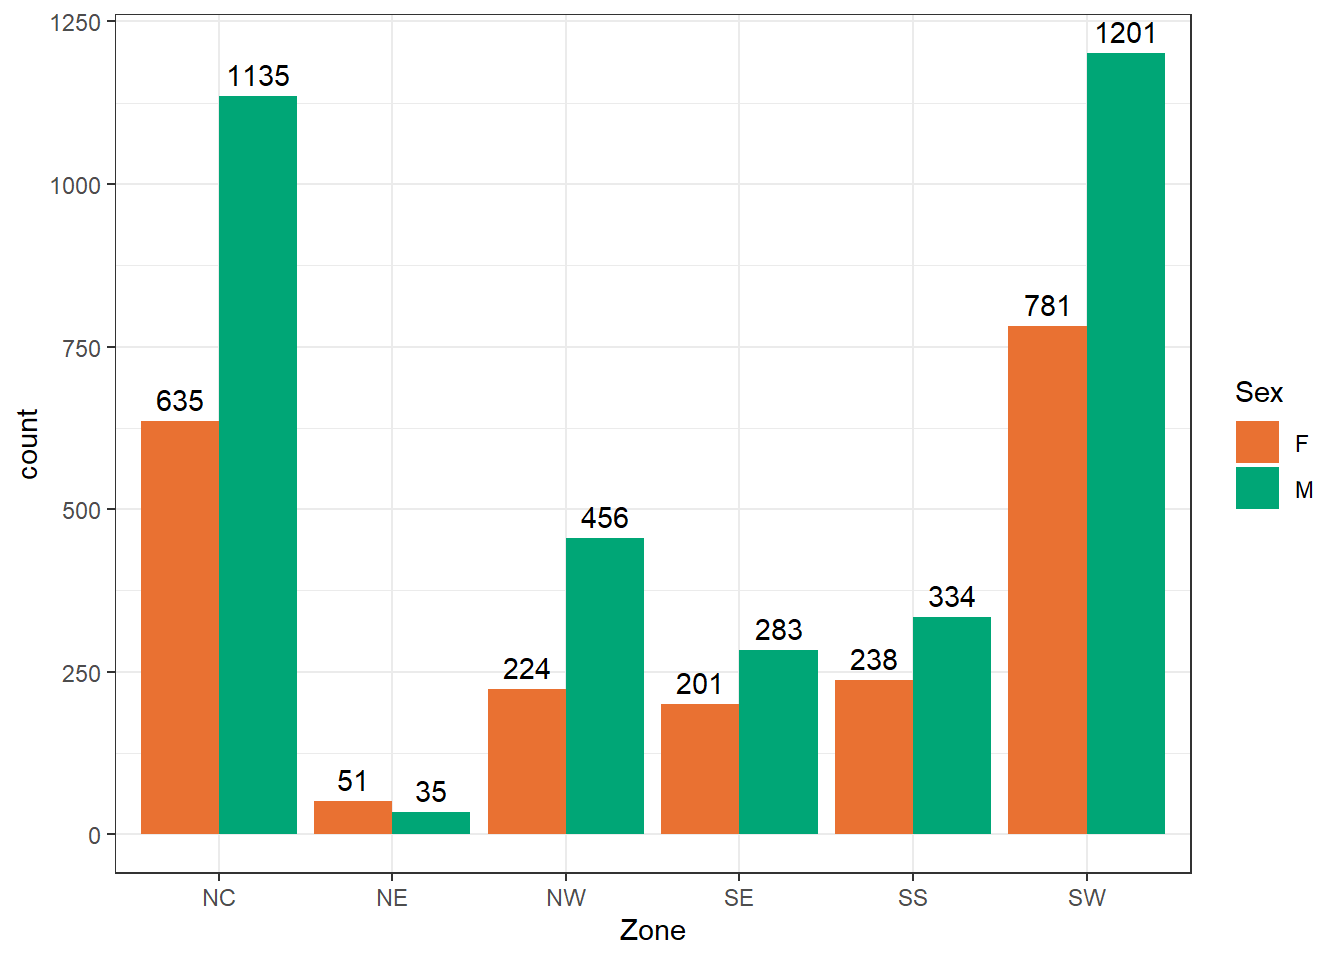
\includegraphics{nationalRR_files/figure-pdf/unnamed-chunk-11-1.pdf}

\subsection{Temporal Trends in Kidney Failure
Pattern}\label{temporal-trends-in-kidney-failure-pattern}

Below shows the visualization of the temporal trends in RRT in Nigeria
(2022 - 2023)

\begin{Shaded}
\begin{Highlighting}[]
\CommentTok{\# Aggregrate dataframe to show monthly trends}

\NormalTok{rr\_data\_new }\SpecialCharTok{\%\textgreater{}\%} 
  \FunctionTok{mutate}\NormalTok{(}\AttributeTok{monthly\_rrt =} \FunctionTok{floor\_date}\NormalTok{(}\StringTok{\textasciigrave{}}\AttributeTok{Date of Diagnosis}\StringTok{\textasciigrave{}}\NormalTok{, }\AttributeTok{unit =} \StringTok{\textquotesingle{}months\textquotesingle{}}\NormalTok{)) }\SpecialCharTok{\%\textgreater{}\%}
  \FunctionTok{group\_by}\NormalTok{(monthly\_rrt) }\SpecialCharTok{\%\textgreater{}\%} 
  \FunctionTok{summarise}\NormalTok{(}\AttributeTok{monthly\_rrt\_pts =} \FunctionTok{n}\NormalTok{()) }\SpecialCharTok{\%\textgreater{}\%} 
  \FunctionTok{filter}\NormalTok{(monthly\_rrt }\SpecialCharTok{\textgreater{}=} \FunctionTok{ymd}\NormalTok{(}\StringTok{\textquotesingle{}2022{-}01{-}01\textquotesingle{}}\NormalTok{) }\SpecialCharTok{\&}\NormalTok{ monthly\_rrt }\SpecialCharTok{\textless{}} \FunctionTok{ymd}\NormalTok{(}\StringTok{\textquotesingle{}2024{-}01{-}01\textquotesingle{}}\NormalTok{)) }\SpecialCharTok{\%\textgreater{}\%} 
  \FunctionTok{ggplot}\NormalTok{()}\SpecialCharTok{+}
  \FunctionTok{geom\_vline}\NormalTok{(}\AttributeTok{xintercept =} \FunctionTok{ymd}\NormalTok{(}\StringTok{\textquotesingle{}2022{-}03{-}01\textquotesingle{}}\NormalTok{), }\AttributeTok{width =}\NormalTok{ .}\DecValTok{1}\NormalTok{, }\AttributeTok{color =} \StringTok{\textquotesingle{}red\textquotesingle{}}\NormalTok{,}
             \AttributeTok{linetype =} \StringTok{\textquotesingle{}dashed\textquotesingle{}}\NormalTok{)}\SpecialCharTok{+}
  \FunctionTok{geom\_vline}\NormalTok{(}\AttributeTok{xintercept =} \FunctionTok{ymd}\NormalTok{(}\StringTok{\textquotesingle{}2022{-}09{-}01\textquotesingle{}}\NormalTok{), }\AttributeTok{width =}\NormalTok{ .}\DecValTok{1}\NormalTok{, }\AttributeTok{color =} \StringTok{\textquotesingle{}red\textquotesingle{}}\NormalTok{,}
             \AttributeTok{linetype =} \StringTok{\textquotesingle{}dashed\textquotesingle{}}\NormalTok{)}\SpecialCharTok{+}
  \FunctionTok{geom\_vline}\NormalTok{(}\AttributeTok{xintercept =} \FunctionTok{ymd}\NormalTok{(}\StringTok{\textquotesingle{}2023{-}03{-}01\textquotesingle{}}\NormalTok{), }\AttributeTok{width =}\NormalTok{ .}\DecValTok{1}\NormalTok{, }\AttributeTok{color =} \StringTok{\textquotesingle{}red\textquotesingle{}}\NormalTok{,}
             \AttributeTok{linetype =} \StringTok{\textquotesingle{}dashed\textquotesingle{}}\NormalTok{)}\SpecialCharTok{+}
  \FunctionTok{geom\_vline}\NormalTok{(}\AttributeTok{xintercept =} \FunctionTok{ymd}\NormalTok{(}\StringTok{\textquotesingle{}2023{-}09{-}01\textquotesingle{}}\NormalTok{), }\AttributeTok{width =}\NormalTok{ .}\DecValTok{1}\NormalTok{, }\AttributeTok{color =} \StringTok{\textquotesingle{}red\textquotesingle{}}\NormalTok{,}
             \AttributeTok{linetype =} \StringTok{\textquotesingle{}dashed\textquotesingle{}}\NormalTok{)}\SpecialCharTok{+}
  \FunctionTok{annotate}\NormalTok{(}\StringTok{\textquotesingle{}text\textquotesingle{}}\NormalTok{,}\AttributeTok{x =} \FunctionTok{ymd}\NormalTok{(}\StringTok{\textquotesingle{}2022{-}06{-}01\textquotesingle{}}\NormalTok{), }\AttributeTok{y =} \DecValTok{650}\NormalTok{, }\AttributeTok{label =} \StringTok{\textquotesingle{}Dry Season\textquotesingle{}}\NormalTok{, }\AttributeTok{size =} \FloatTok{3.5}\NormalTok{)}\SpecialCharTok{+}
  \FunctionTok{annotate}\NormalTok{(}\StringTok{\textquotesingle{}text\textquotesingle{}}\NormalTok{,}\AttributeTok{x =} \FunctionTok{ymd}\NormalTok{(}\StringTok{\textquotesingle{}2022{-}12{-}01\textquotesingle{}}\NormalTok{), }\AttributeTok{y =} \DecValTok{650}\NormalTok{, }\AttributeTok{label =} \StringTok{\textquotesingle{}Wet Season\textquotesingle{}}\NormalTok{, }\AttributeTok{size =} \FloatTok{3.5}\NormalTok{)}\SpecialCharTok{+}
  \FunctionTok{annotate}\NormalTok{(}\StringTok{\textquotesingle{}text\textquotesingle{}}\NormalTok{,}\AttributeTok{x =} \FunctionTok{ymd}\NormalTok{(}\StringTok{\textquotesingle{}2023{-}06{-}01\textquotesingle{}}\NormalTok{), }\AttributeTok{y =} \DecValTok{650}\NormalTok{, }\AttributeTok{label =} \StringTok{\textquotesingle{}Dry Season\textquotesingle{}}\NormalTok{, }\AttributeTok{size =} \FloatTok{3.5}\NormalTok{)}\SpecialCharTok{+}
  \FunctionTok{geom\_line}\NormalTok{(}\FunctionTok{aes}\NormalTok{(}\AttributeTok{x =}\NormalTok{ monthly\_rrt, }\AttributeTok{y =}\NormalTok{ monthly\_rrt\_pts), }\AttributeTok{color =} \StringTok{"\#00A676"}\NormalTok{, }\AttributeTok{width =} \DecValTok{2}\NormalTok{)}\SpecialCharTok{+}
  \FunctionTok{labs}\NormalTok{(}\AttributeTok{title =} \StringTok{\textquotesingle{}Temporal trends in Renal Failure Incidence\textquotesingle{}}\NormalTok{,}
       \AttributeTok{x =} \StringTok{\textquotesingle{}Monthly Trend\textquotesingle{}}\NormalTok{,}
       \AttributeTok{y=} \StringTok{\textquotesingle{}No of Patients\textquotesingle{}}\NormalTok{)}\SpecialCharTok{+}
  \FunctionTok{theme\_bw}\NormalTok{()}
\end{Highlighting}
\end{Shaded}

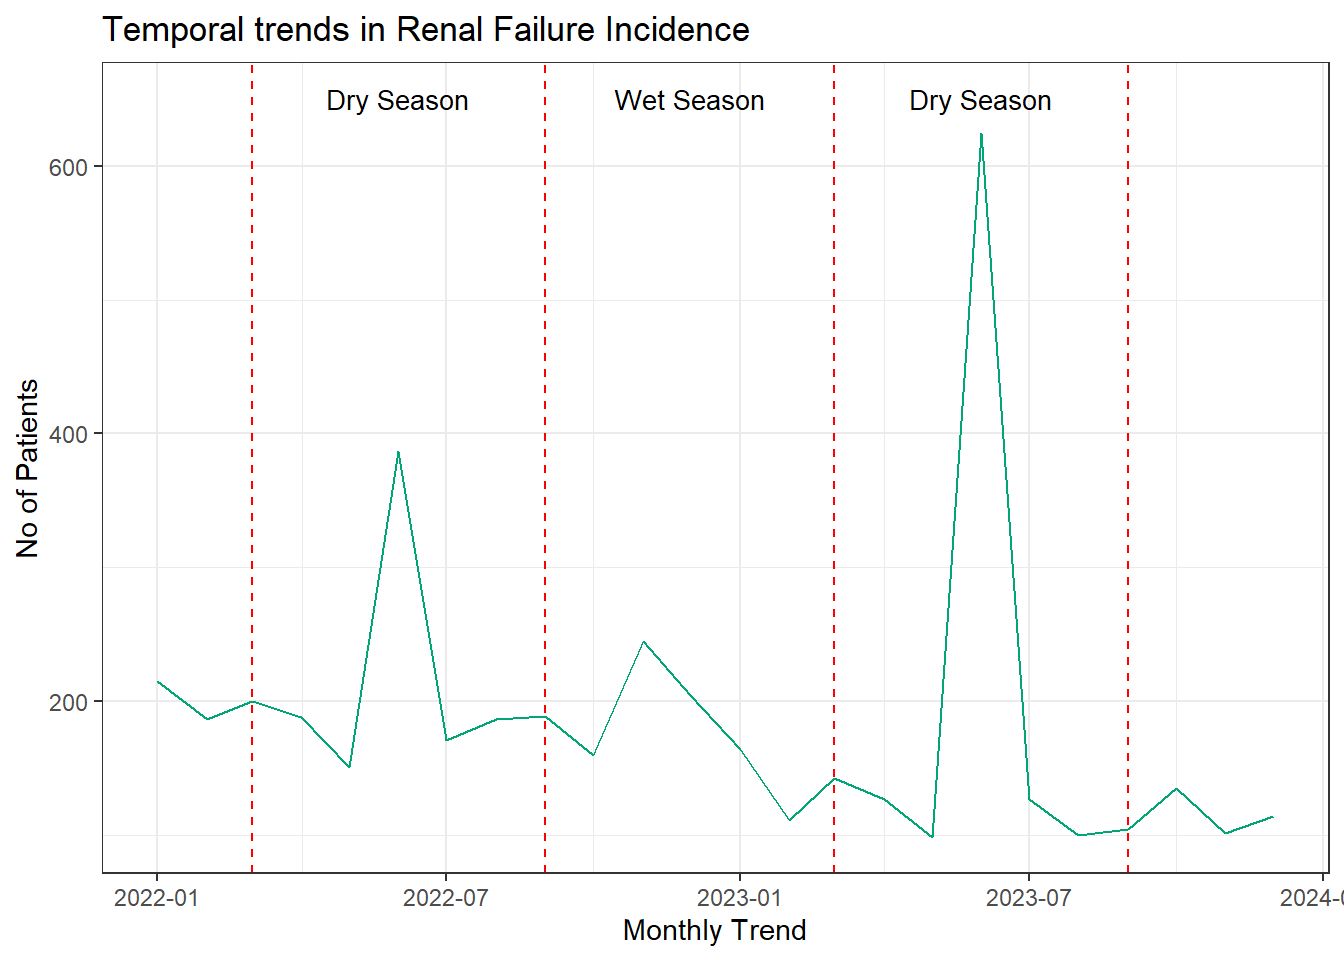
\includegraphics{nationalRR_files/figure-pdf/unnamed-chunk-12-1.pdf}

\subsection{Vascular Access (Overall and by
Zone)}\label{vascular-access-overall-and-by-zone}

\begin{Shaded}
\begin{Highlighting}[]
\CommentTok{\# Overall Vascular Access}
\NormalTok{rr\_data\_new }\SpecialCharTok{\%\textgreater{}\%}
  \FunctionTok{filter}\NormalTok{(}\StringTok{\textasciigrave{}}\AttributeTok{Vascular Access}\StringTok{\textasciigrave{}} \SpecialCharTok{\%in\%} \FunctionTok{c}\NormalTok{(}\StringTok{\textquotesingle{}AV Fistula\textquotesingle{}}\NormalTok{,}\StringTok{\textquotesingle{}Temporary Femoral Catheter\textquotesingle{}}\NormalTok{,}
                                  \StringTok{\textquotesingle{}Tunneled CVC\textquotesingle{}}\NormalTok{)) }\SpecialCharTok{\%\textgreater{}\%} 
  \FunctionTok{select}\NormalTok{(}\StringTok{\textasciigrave{}}\AttributeTok{Vascular Access}\StringTok{\textasciigrave{}}\NormalTok{) }\SpecialCharTok{\%\textgreater{}\%} 
  \FunctionTok{group\_by}\NormalTok{(}\StringTok{\textasciigrave{}}\AttributeTok{Vascular Access}\StringTok{\textasciigrave{}}\NormalTok{) }\SpecialCharTok{\%\textgreater{}\%} 
  \FunctionTok{summarise}\NormalTok{(}\AttributeTok{count =} \FunctionTok{n}\NormalTok{(),}
         \StringTok{\textasciigrave{}}\AttributeTok{\%Vascular Access}\StringTok{\textasciigrave{}} \OtherTok{=} \FunctionTok{paste0}\NormalTok{(}\FunctionTok{round}\NormalTok{((count}\SpecialCharTok{/}\DecValTok{4850}\NormalTok{)}\SpecialCharTok{*}\DecValTok{100}\NormalTok{, }\DecValTok{1}\NormalTok{),}\StringTok{\textquotesingle{}\%\textquotesingle{}}\NormalTok{))}
\end{Highlighting}
\end{Shaded}

\begin{verbatim}
# A tibble: 3 x 3
  `Vascular Access`          count `%Vascular Access`
  <fct>                      <int> <chr>             
1 AV Fistula                   102 2.1%              
2 Temporary Femoral Catheter  3228 66.6%             
3 Tunneled CVC                1520 31.3%             
\end{verbatim}

\begin{Shaded}
\begin{Highlighting}[]
\NormalTok{rr\_data\_new }\SpecialCharTok{\%\textgreater{}\%} 
  \FunctionTok{filter}\NormalTok{(}\StringTok{\textasciigrave{}}\AttributeTok{Vascular Access}\StringTok{\textasciigrave{}} \SpecialCharTok{\%in\%} \FunctionTok{c}\NormalTok{(}\StringTok{\textquotesingle{}AV Fistula\textquotesingle{}}\NormalTok{,}\StringTok{\textquotesingle{}Temporary Femoral Catheter\textquotesingle{}}\NormalTok{,}
                                  \StringTok{\textquotesingle{}Tunneled CVC\textquotesingle{}}\NormalTok{)) }\SpecialCharTok{\%\textgreater{}\%}
  \FunctionTok{ggplot}\NormalTok{(}\FunctionTok{aes}\NormalTok{(}\AttributeTok{x =}\NormalTok{ Zone, }\AttributeTok{fill =} \StringTok{\textasciigrave{}}\AttributeTok{Vascular Access}\StringTok{\textasciigrave{}}\NormalTok{)) }\SpecialCharTok{+}
  \FunctionTok{geom\_bar}\NormalTok{(}\AttributeTok{position =} \StringTok{\textquotesingle{}fill\textquotesingle{}}\NormalTok{)}\SpecialCharTok{+}
  \FunctionTok{scale\_fill\_manual}\NormalTok{(}\AttributeTok{values =} \FunctionTok{c}\NormalTok{(}\StringTok{"AV Fistula"} \OtherTok{=} \StringTok{"\#E97132"}\NormalTok{,}
                              \StringTok{"Temporary Femoral Catheter"} \OtherTok{=} \StringTok{"\#00A676"}\NormalTok{,}
                              \StringTok{"Tunneled CVC"} \OtherTok{=} \StringTok{"\#FFC000"}\NormalTok{))}\SpecialCharTok{+}
  \FunctionTok{labs}\NormalTok{(}\AttributeTok{title =} \StringTok{\textquotesingle{}Vascular Access by Zone\textquotesingle{}}\NormalTok{,}
       \AttributeTok{y =} \StringTok{\textquotesingle{}Percentage of total in zone\textquotesingle{}}\NormalTok{)}\SpecialCharTok{+}
  \FunctionTok{theme\_bw}\NormalTok{()}
\end{Highlighting}
\end{Shaded}

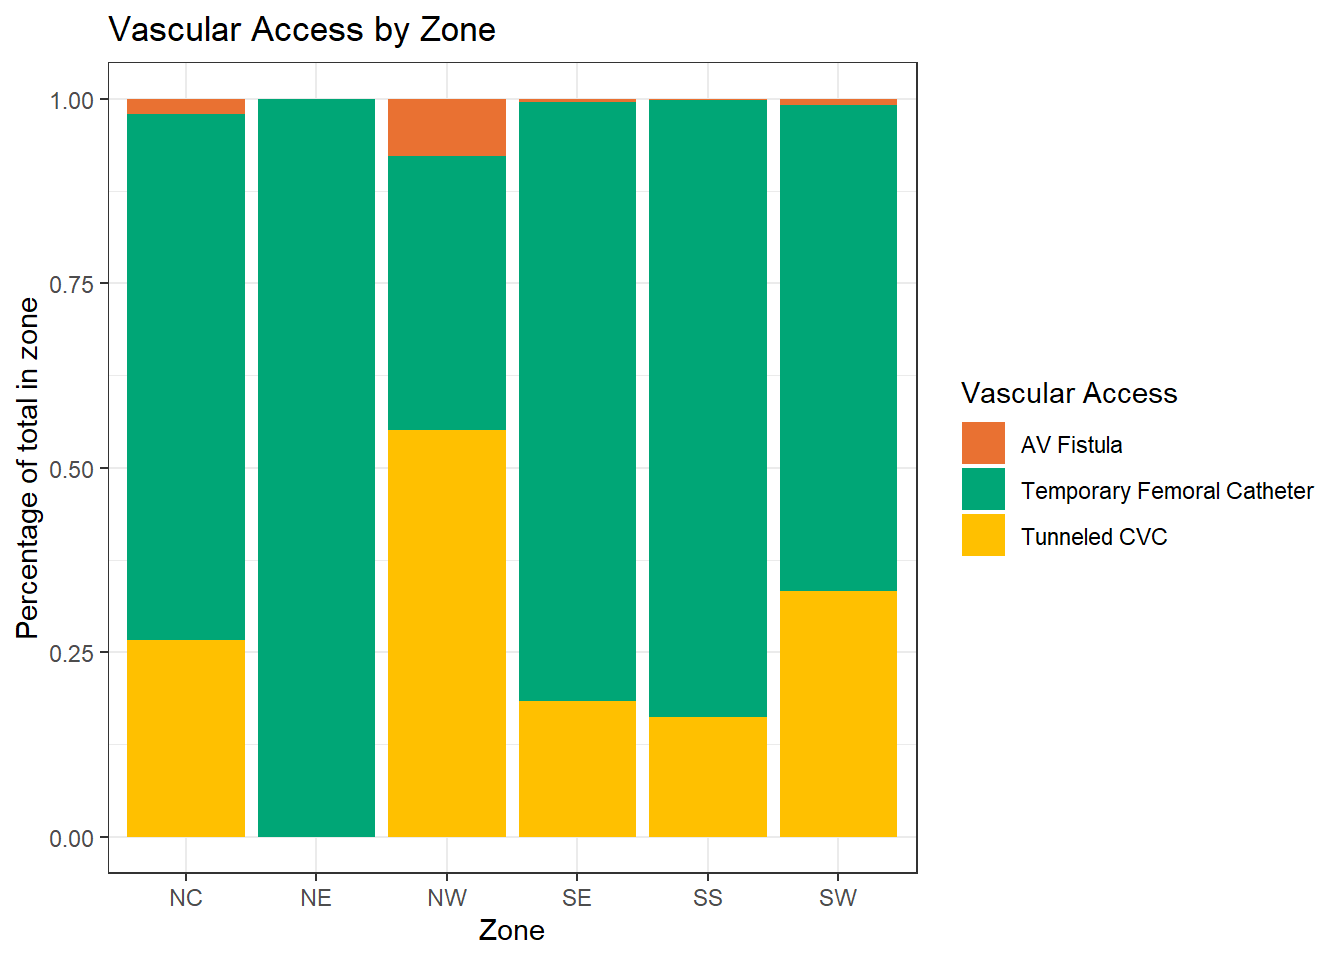
\includegraphics{nationalRR_files/figure-pdf/unnamed-chunk-14-1.pdf}

\subsection{Health Outcomes (by Zone)}\label{health-outcomes-by-zone}

\begin{Shaded}
\begin{Highlighting}[]
\NormalTok{rr\_data\_new }\SpecialCharTok{\%\textgreater{}\%} 
  \FunctionTok{filter}\NormalTok{(Outcome }\SpecialCharTok{\%in\%} \FunctionTok{c}\NormalTok{(}\StringTok{\textquotesingle{}Dead\textquotesingle{}}\NormalTok{,}\StringTok{\textquotesingle{}Transplant\textquotesingle{}}\NormalTok{,}\StringTok{\textquotesingle{}Alive\textquotesingle{}}\NormalTok{)) }\SpecialCharTok{\%\textgreater{}\%}
  \FunctionTok{ggplot}\NormalTok{(}\FunctionTok{aes}\NormalTok{(}\AttributeTok{y =}\NormalTok{ Zone, }\AttributeTok{fill =}\NormalTok{ Outcome)) }\SpecialCharTok{+}
  \FunctionTok{geom\_bar}\NormalTok{(}\AttributeTok{position =} \StringTok{\textquotesingle{}fill\textquotesingle{}}\NormalTok{)}\SpecialCharTok{+}
  \FunctionTok{scale\_fill\_manual}\NormalTok{(}\AttributeTok{values =} \FunctionTok{c}\NormalTok{(}\StringTok{"Dead"} \OtherTok{=} \StringTok{"\#E97132"}\NormalTok{,}
                              \StringTok{"Alive"} \OtherTok{=} \StringTok{"\#00A676"}\NormalTok{,}
                              \StringTok{"Transplant"} \OtherTok{=} \StringTok{"\#FFC000"}\NormalTok{))}\SpecialCharTok{+}
  \FunctionTok{labs}\NormalTok{(}\AttributeTok{title =} \StringTok{\textquotesingle{}Outcomes by Zone\textquotesingle{}}\NormalTok{,}
       \AttributeTok{x =} \StringTok{\textquotesingle{}Percentage of total in zone\textquotesingle{}}\NormalTok{)}\SpecialCharTok{+}
  \FunctionTok{theme\_bw}\NormalTok{()}
\end{Highlighting}
\end{Shaded}

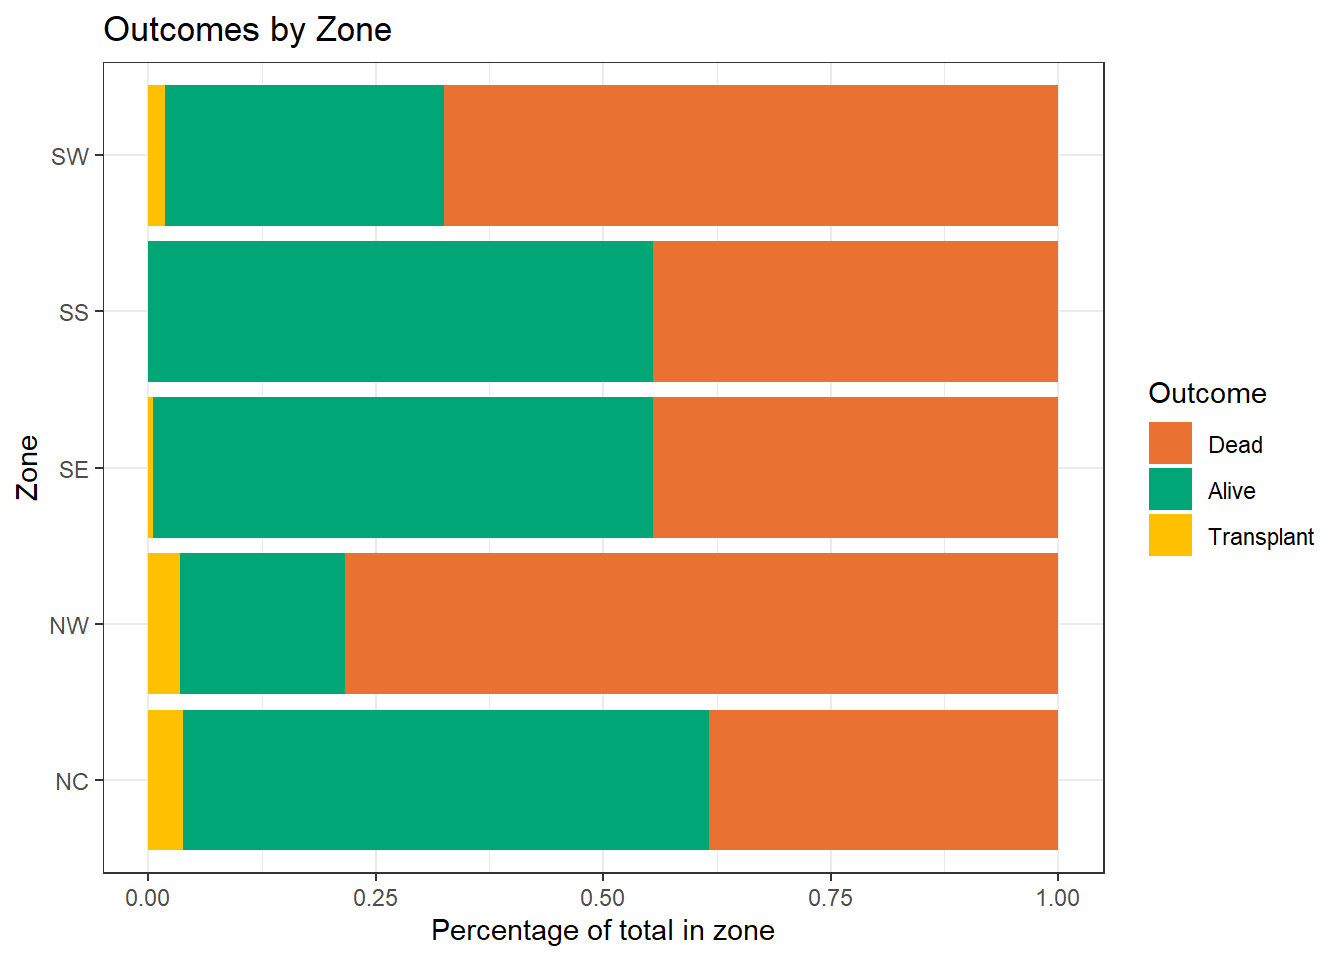
\includegraphics{nationalRR_files/figure-pdf/unnamed-chunk-15-1.pdf}

\subsection{Survival Analysis of Various Factors influencing Time to
death}\label{survival-analysis-of-various-factors-influencing-time-to-death}

\begin{Shaded}
\begin{Highlighting}[]
\CommentTok{\# Extract df for sample survival analysis for variable HIV}

\NormalTok{HIV\_survival\_data }\OtherTok{\textless{}{-}}\NormalTok{ rr\_data\_new }\SpecialCharTok{\%\textgreater{}\%}
  \FunctionTok{filter}\NormalTok{(}\StringTok{\textasciigrave{}}\AttributeTok{Date of Diagnosis}\StringTok{\textasciigrave{}} \SpecialCharTok{\textgreater{}} \FunctionTok{ymd}\NormalTok{(}\StringTok{\textquotesingle{}2022{-}01{-}01\textquotesingle{}}\NormalTok{) }\SpecialCharTok{\&}
           \StringTok{\textasciigrave{}}\AttributeTok{Date of Diagnosis}\StringTok{\textasciigrave{}} \SpecialCharTok{\%{-}{-}\%} \StringTok{\textasciigrave{}}\AttributeTok{Date of Death or Transplant}\StringTok{\textasciigrave{}}\SpecialCharTok{/}\FunctionTok{days}\NormalTok{() }\SpecialCharTok{\textgreater{}} \DecValTok{0}\NormalTok{ ) }\SpecialCharTok{\%\textgreater{}\%}
  \FunctionTok{filter}\NormalTok{(HIV }\SpecialCharTok{\%in\%} \FunctionTok{c}\NormalTok{(}\StringTok{\textquotesingle{}Pos\textquotesingle{}}\NormalTok{, }\StringTok{\textquotesingle{}Neg\textquotesingle{}}\NormalTok{)) }\SpecialCharTok{\%\textgreater{}\%} 
  \FunctionTok{mutate}\NormalTok{(}\StringTok{\textasciigrave{}}\AttributeTok{HIV status}\StringTok{\textasciigrave{}} \OtherTok{=} \FunctionTok{case\_when}\NormalTok{(HIV }\SpecialCharTok{==} \StringTok{\textquotesingle{}Neg\textquotesingle{}}\SpecialCharTok{\textasciitilde{}} \DecValTok{0}\NormalTok{,}
\NormalTok{                                    HIV }\SpecialCharTok{==} \StringTok{\textquotesingle{}Pos\textquotesingle{}}\SpecialCharTok{\textasciitilde{}} \DecValTok{1}\NormalTok{),}
           \AttributeTok{days =} \StringTok{\textasciigrave{}}\AttributeTok{Date of Diagnosis}\StringTok{\textasciigrave{}} \SpecialCharTok{\%{-}{-}\%} \StringTok{\textasciigrave{}}\AttributeTok{Date of Death or Transplant}\StringTok{\textasciigrave{}}\SpecialCharTok{/}\FunctionTok{days}\NormalTok{(),}
           \StringTok{\textasciigrave{}}\AttributeTok{death status}\StringTok{\textasciigrave{}} \OtherTok{=} \FunctionTok{case\_when}\NormalTok{(Outcome }\SpecialCharTok{==} \StringTok{\textquotesingle{}Dead\textquotesingle{}} \SpecialCharTok{\textasciitilde{}} \DecValTok{1}\NormalTok{,}
\NormalTok{                                      Outcome }\SpecialCharTok{\%in\%} \FunctionTok{c}\NormalTok{(}\StringTok{\textquotesingle{}Alive\textquotesingle{}}\NormalTok{,}\StringTok{\textquotesingle{}Transplant\textquotesingle{}}\NormalTok{) }\SpecialCharTok{\textasciitilde{}} \DecValTok{0}\NormalTok{)) }\SpecialCharTok{\%\textgreater{}\%} 
  \FunctionTok{select}\NormalTok{(days, }\StringTok{\textasciigrave{}}\AttributeTok{HIV status}\StringTok{\textasciigrave{}}\NormalTok{, }\StringTok{\textasciigrave{}}\AttributeTok{death status}\StringTok{\textasciigrave{}}\NormalTok{)}
\end{Highlighting}
\end{Shaded}

\subsection{Hazard Ratios}\label{hazard-ratios}

\section{Key Findings and Discussion}\label{key-findings-and-discussion}

Kindly check the \texttt{.ppt} PowerPoint slides and report for details




\end{document}
